\documentclass{article}

\usepackage{a4wide}
\usepackage{graphicx}
\usepackage{paralist}

\setlength{\parindent}{0em}
\setlength{\parskip}{1em}

\title{Project Information Security 2012}
\author{Pieter De Baets, Gilles Jacobs, Jasper Van der Jeugt, Toon Willems}

\begin{document}

\maketitle
\tableofcontents

\newpage

\section{Requirements and Architecture}

We chose to design system with a central component, i.e., a server, to which the
different clients can connect. One disadvantage of this approach is that this
server needs to be trusted to some extent---which we tried to limit as much as
possible, more on this later---by the users.

\subsection{Assumptions}

We need to assume that every user (students as well as professors) are
registered on this platform. These accounts can be created when a student
enrolls in the institute, or when a professor is employed.

The users of the platform should be able to verify that they are actually
talking to the platform, and not some malicious individual posing as the
platform. Since we will use HTTPS for all communication, this should not be a
problem.

We use an asymptotic encryption mechanism for many features, so we also need to
assume that each user has a keypair assigned. These keypairs can be created at
the same time as the accounts, with some option to reset a keypair when it has
been compromised.

\subsection{Functionality}

\subsubsection{Logging in}

Users (students and professors) should be able to log in to the application.
This means we need some kind of authentication: it is obvious that a student
should not be able to pose as a professor.

\subsubsection{Distributing exams}

The professor needs to be able to distribute an exam to the students. He first
uploads it to the central server, and selects a number of students. These
students can download it from there, at some point in time, also specified by
the professor.

Integrity is important here: we must ensure the students see the same exam that
the professor posted. Furthermore, only the selected students should be able to
see the exam, and we have to make sure they cannot view the exam before they are
allowed to.

\subsection{Expected attacks}

How will attackers try to compromise our system? Why will they fail?

\subsection{Limitations}

In what ways is our system not protected? What do we need to trust?

\section{Practical considerations}

Is it practically feasible to lock up a few dozen students in a small room for a
few days, without food or water?

\section{Concrete implementation}

Some implementation details, we should mention the actually used algorithms
here.

\section{Conclusion}

\section{Images}

A picture is worth a thousand words.

\begin{figure}
\begin{center}
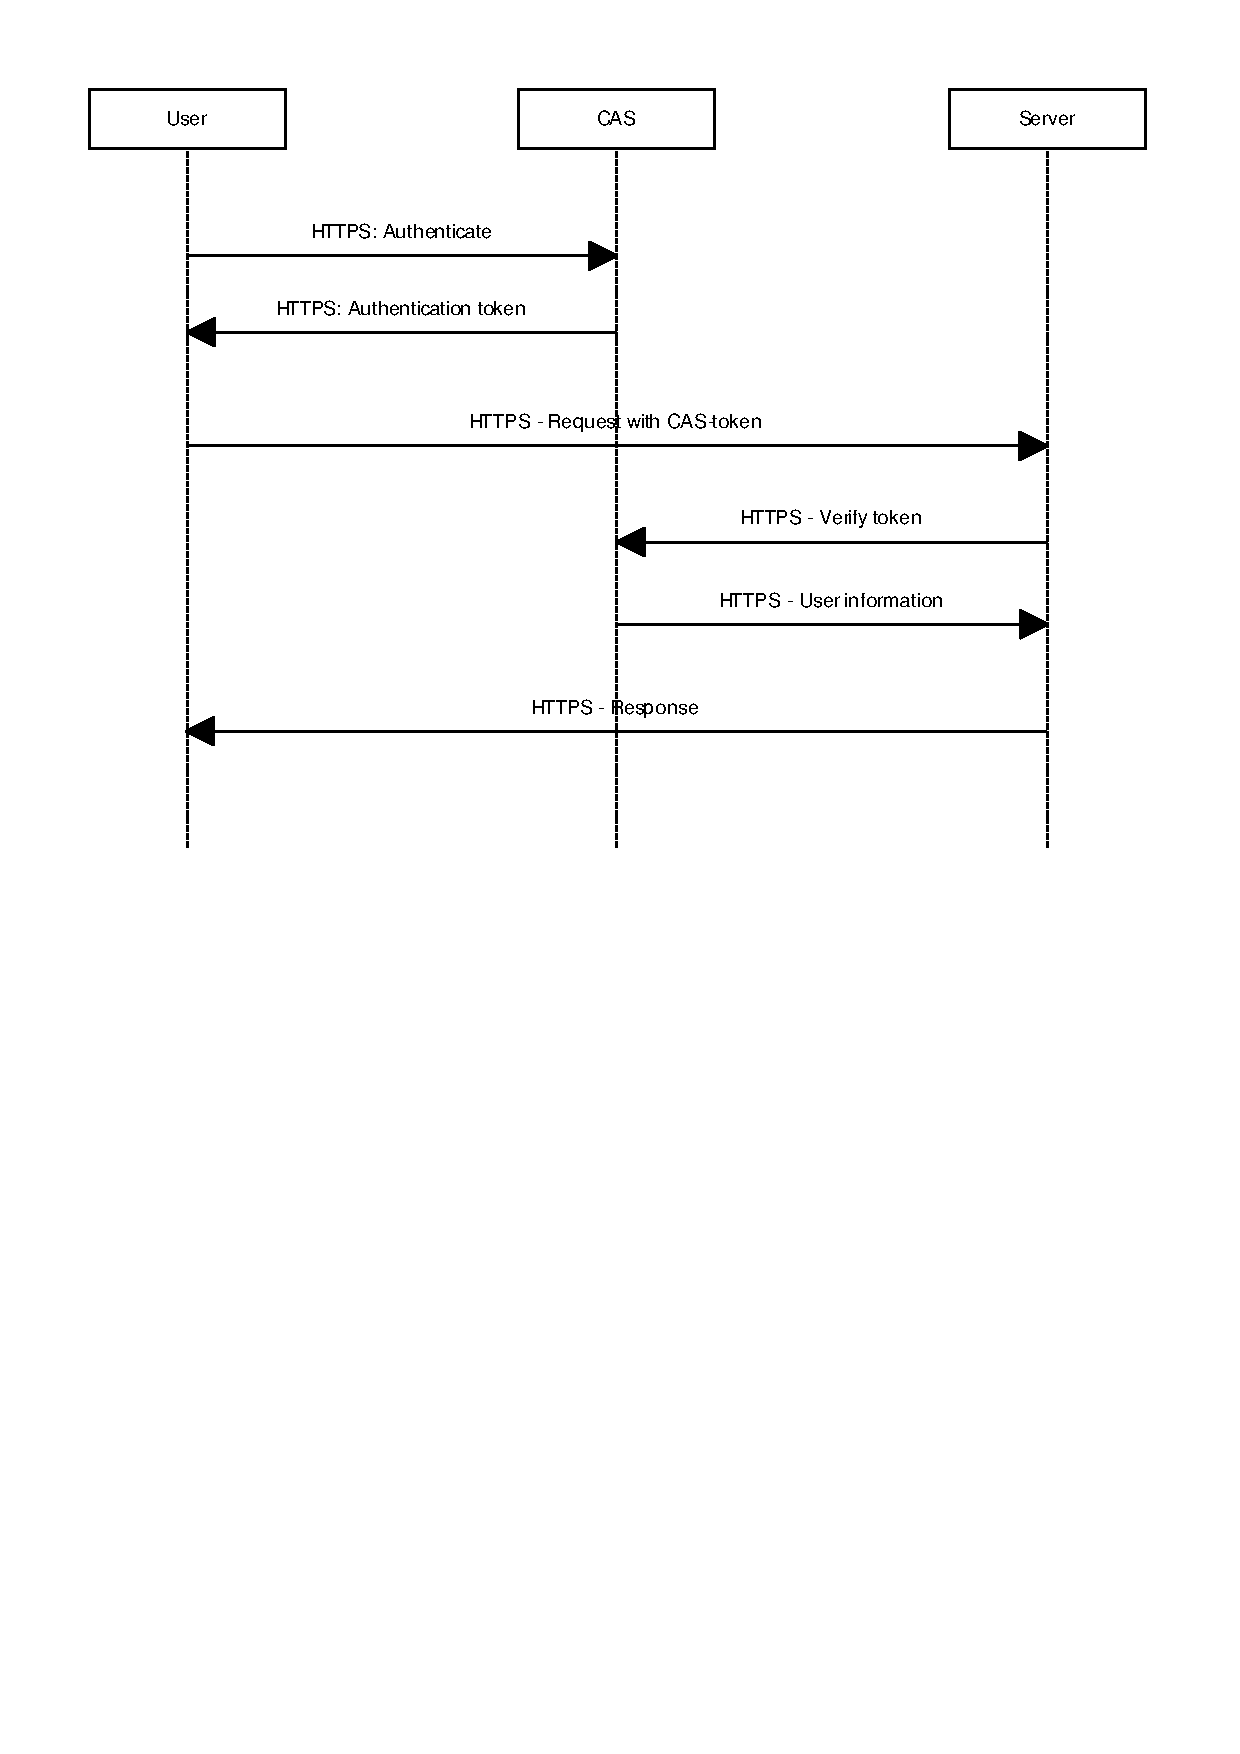
\includegraphics[width=\textwidth]{images/login.pdf}
\caption{Messages exchanged when logging in}
\label{fig:log-in}
\end{center}
\end{figure}

\begin{figure}
\begin{center}
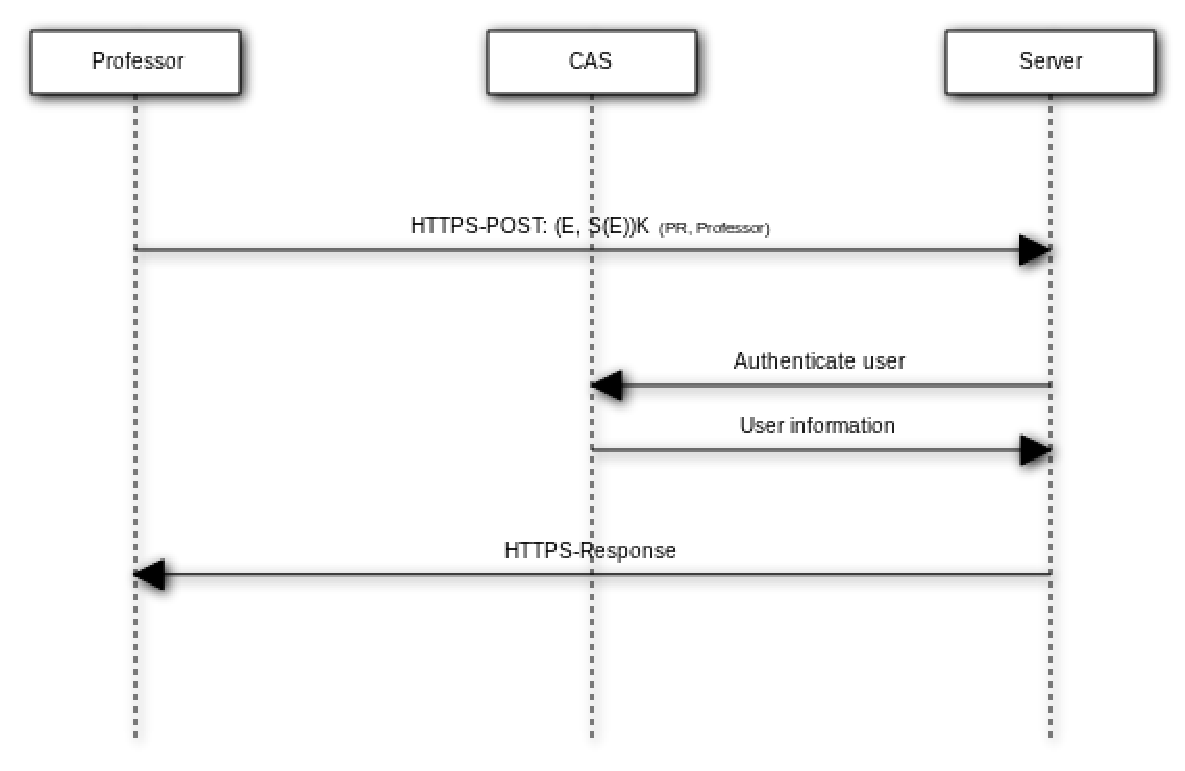
\includegraphics[width=\textwidth]{images/upload_exam.pdf}
\caption{Messages exchanged when uploading an exam}
\label{fig:log-in}
\end{center}
\end{figure}

\begin{figure}
\begin{center}
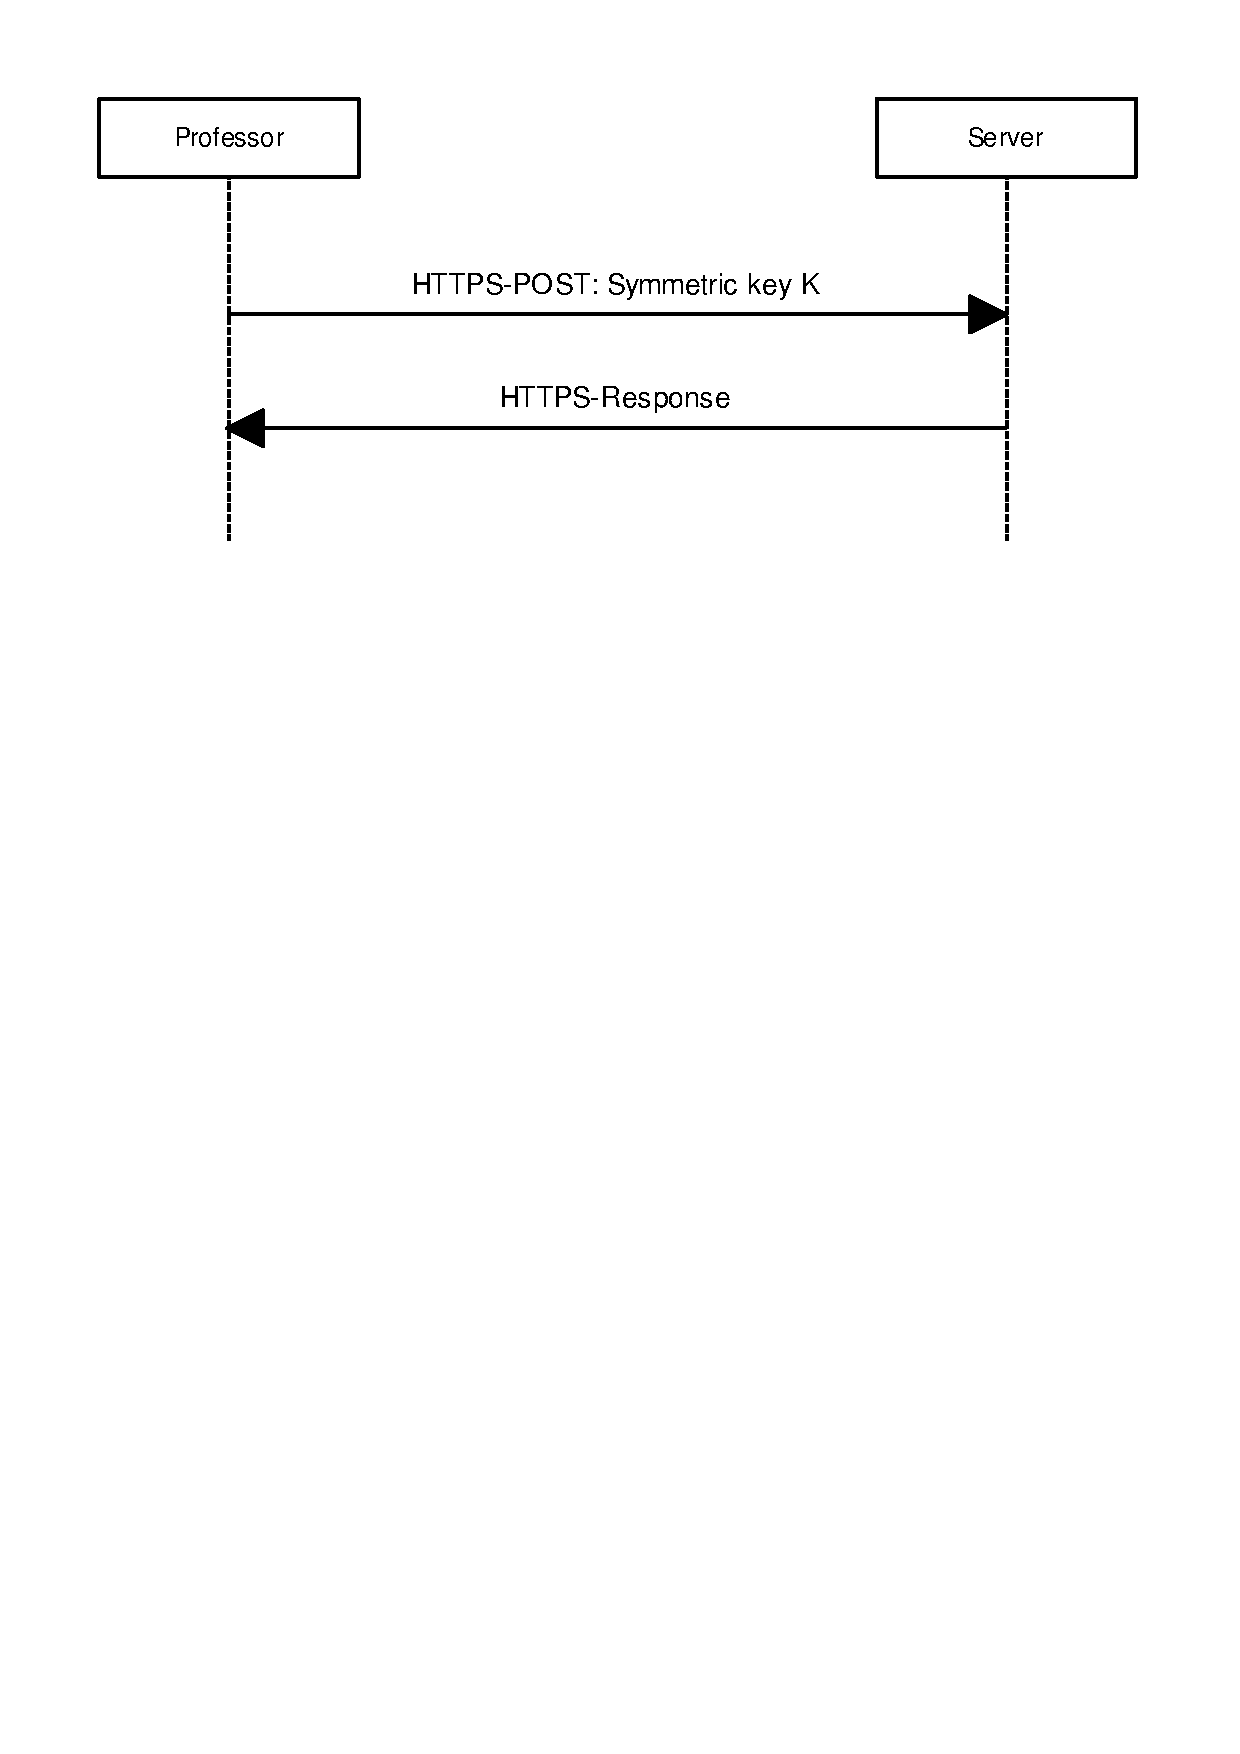
\includegraphics[width=\textwidth]{images/unlock_exam.pdf}
\caption{Messages exchanged when unlocking an exam}
\label{fig:log-in}
\end{center}
\end{figure}

\begin{figure}
\begin{center}
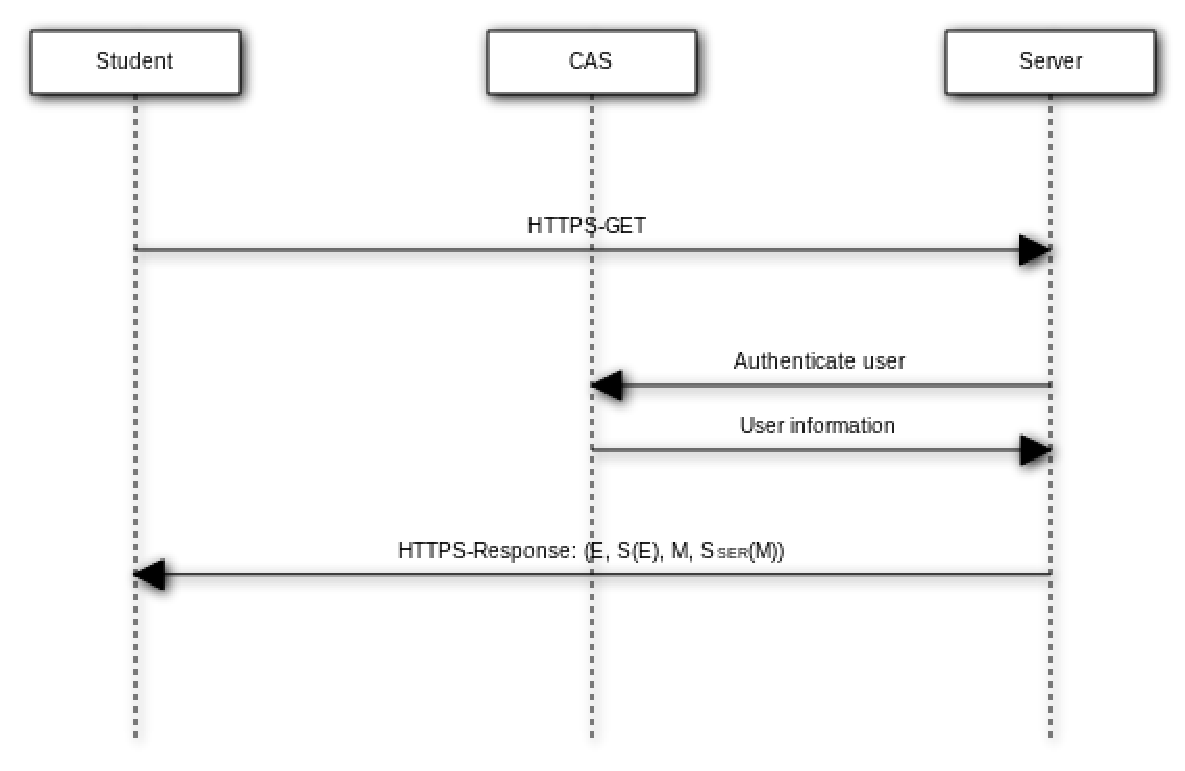
\includegraphics[width=\textwidth]{images/download_exam.pdf}
\caption{Messages exchanged when downloading an exam}
\label{fig:log-in}
\end{center}
\end{figure}

\begin{figure}
\begin{center}
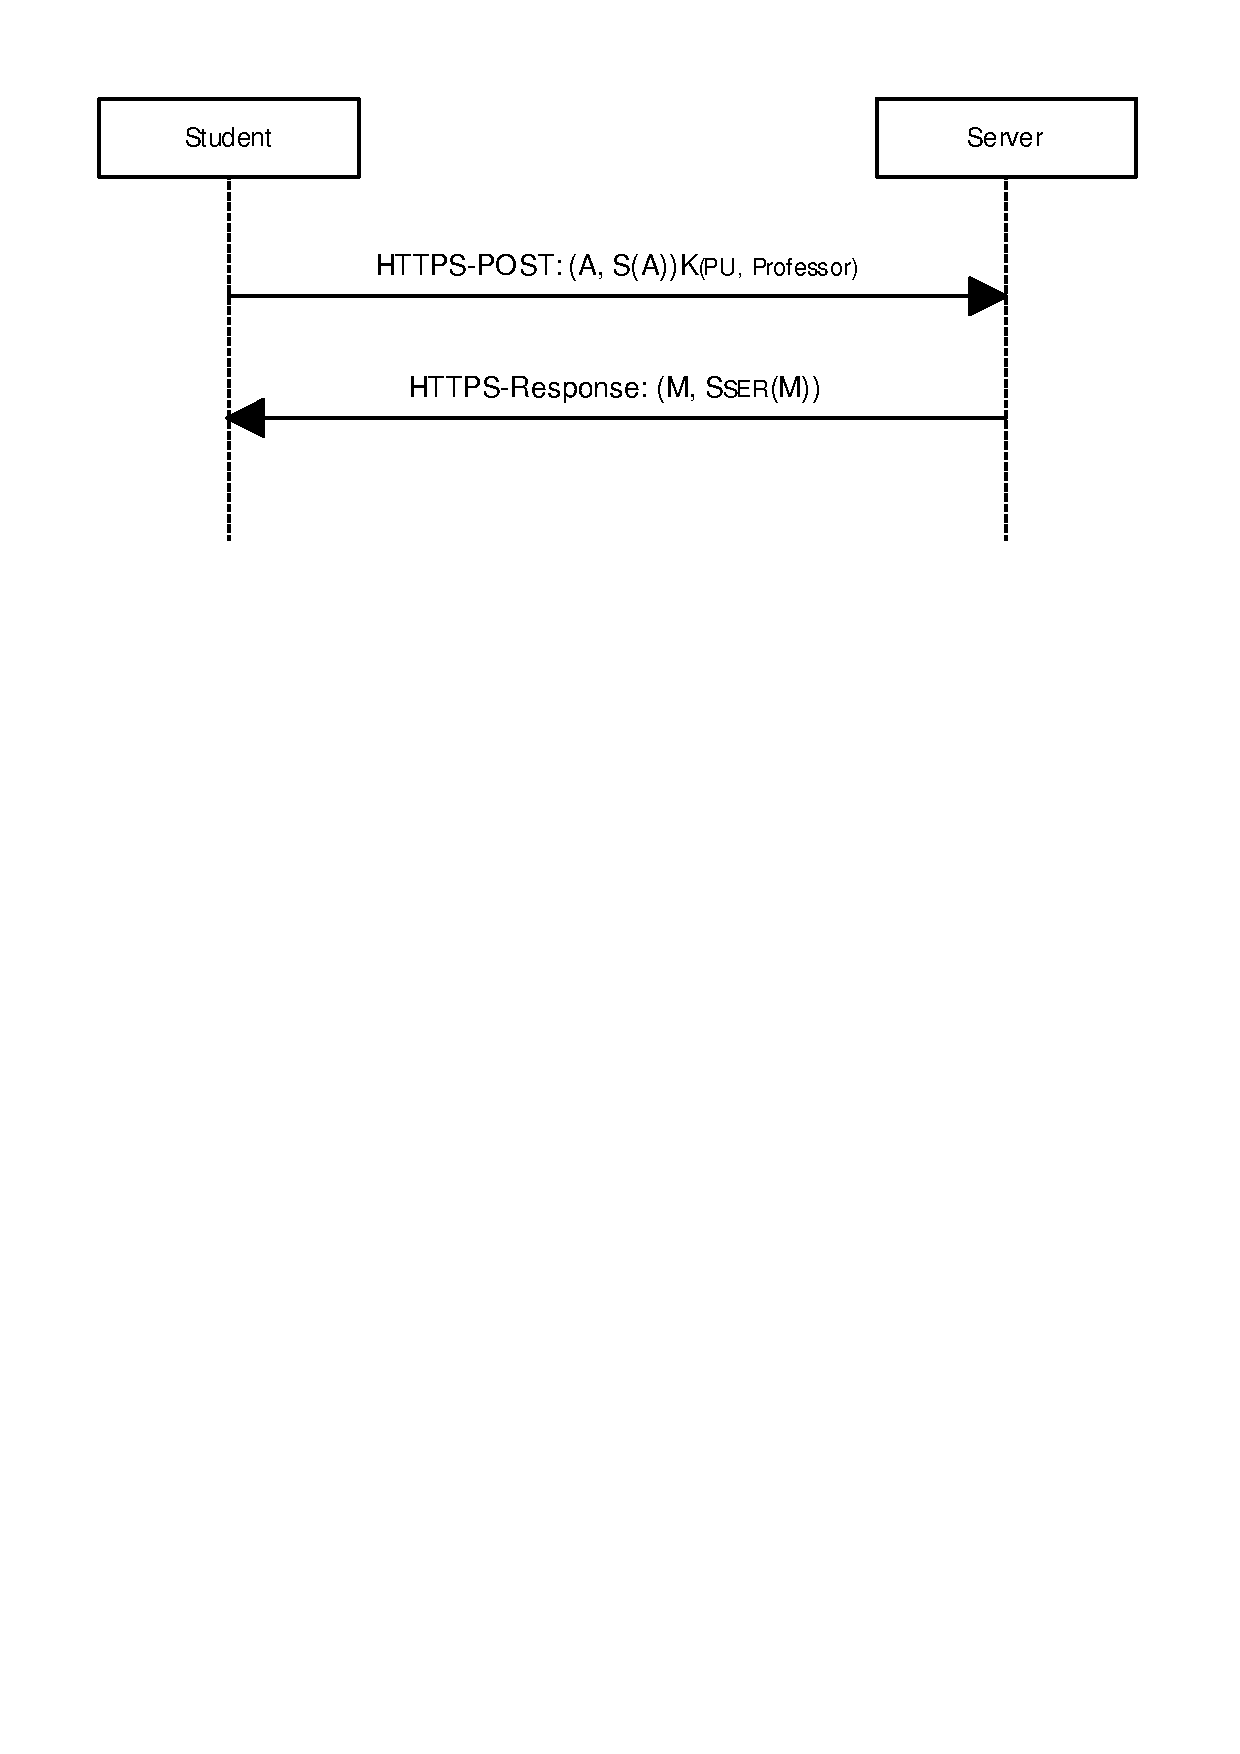
\includegraphics[width=\textwidth]{images/upload_answers.pdf}
\caption{Messages exchanged when uploading answers}
\label{fig:log-in}
\end{center}
\end{figure}

\begin{figure}
\begin{center}
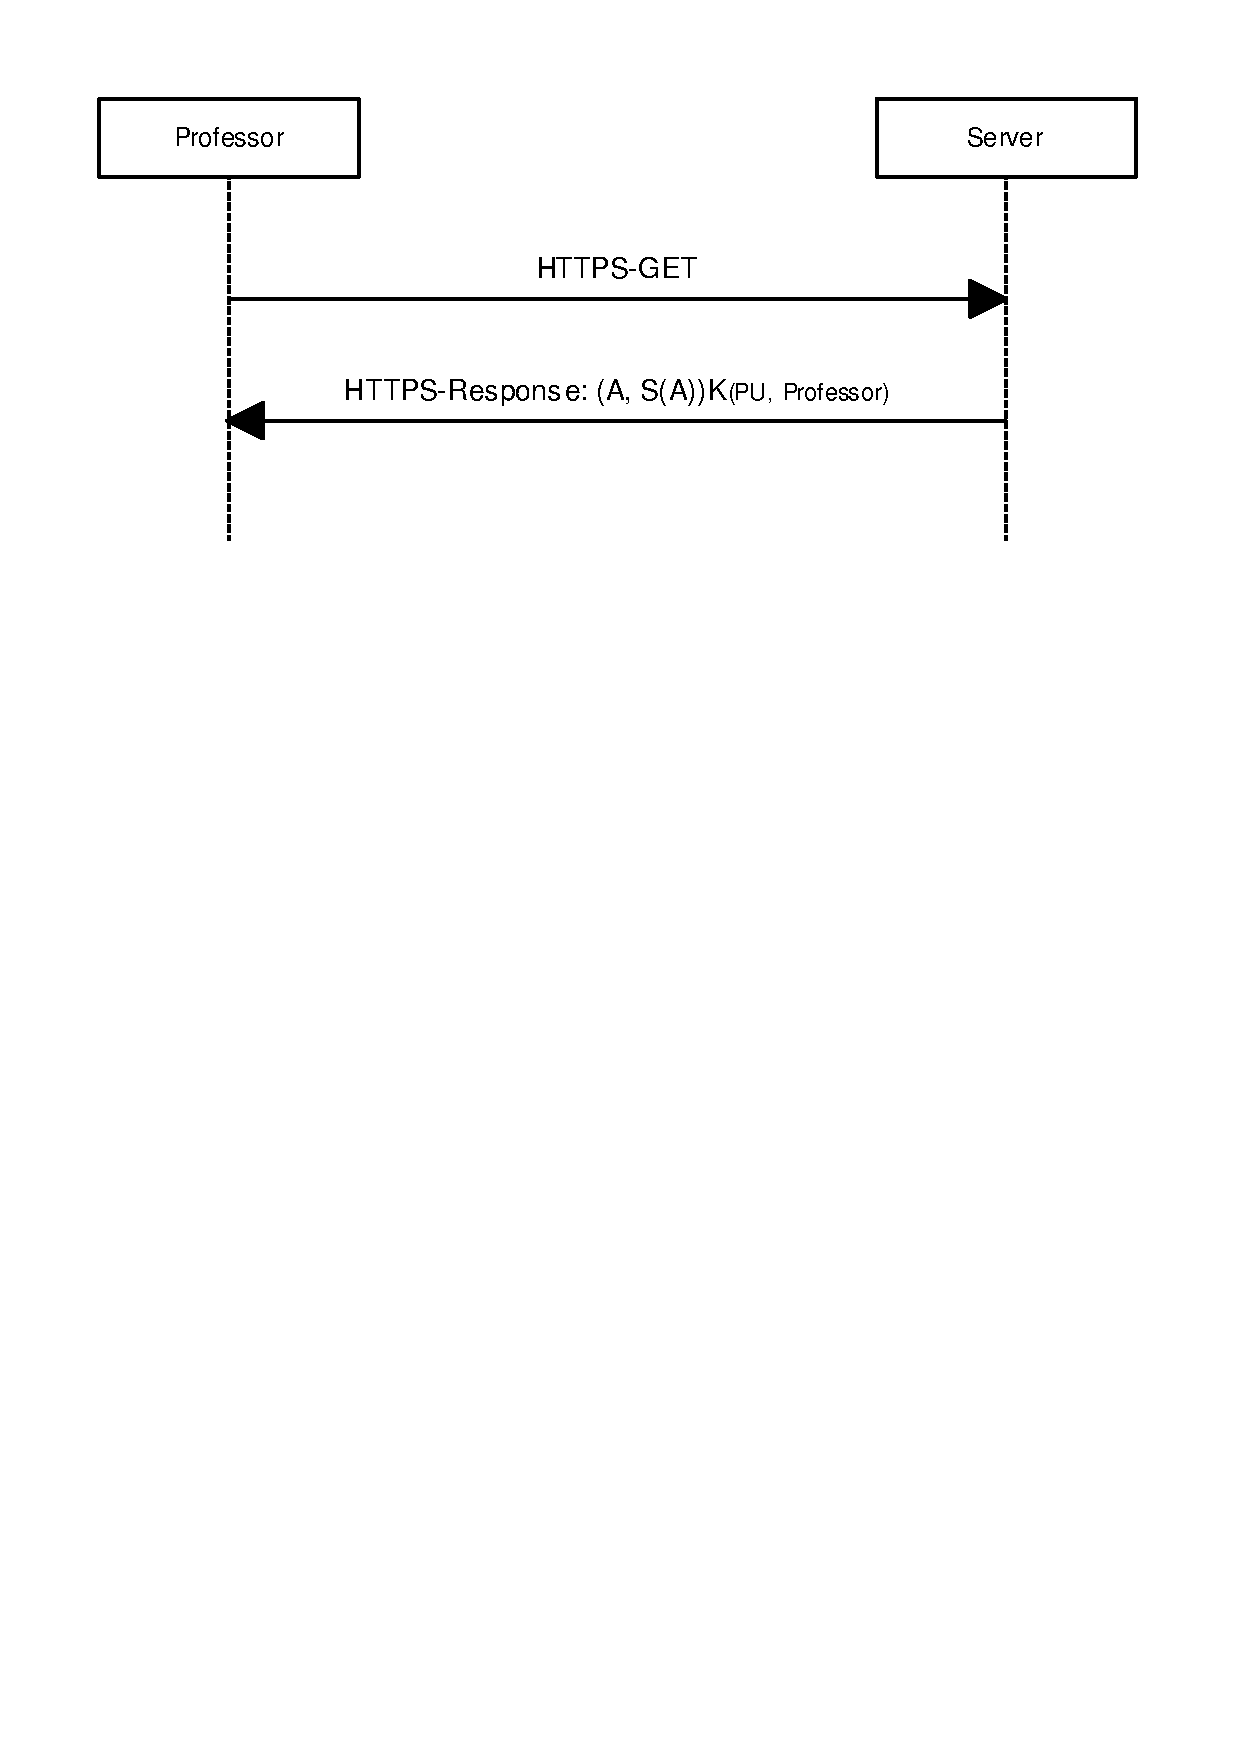
\includegraphics[width=\textwidth]{images/download_answers.pdf}
\caption{Messages exchanged when downloading answers}
\label{fig:log-in}
\end{center}
\end{figure}

\begin{figure}
\begin{center}
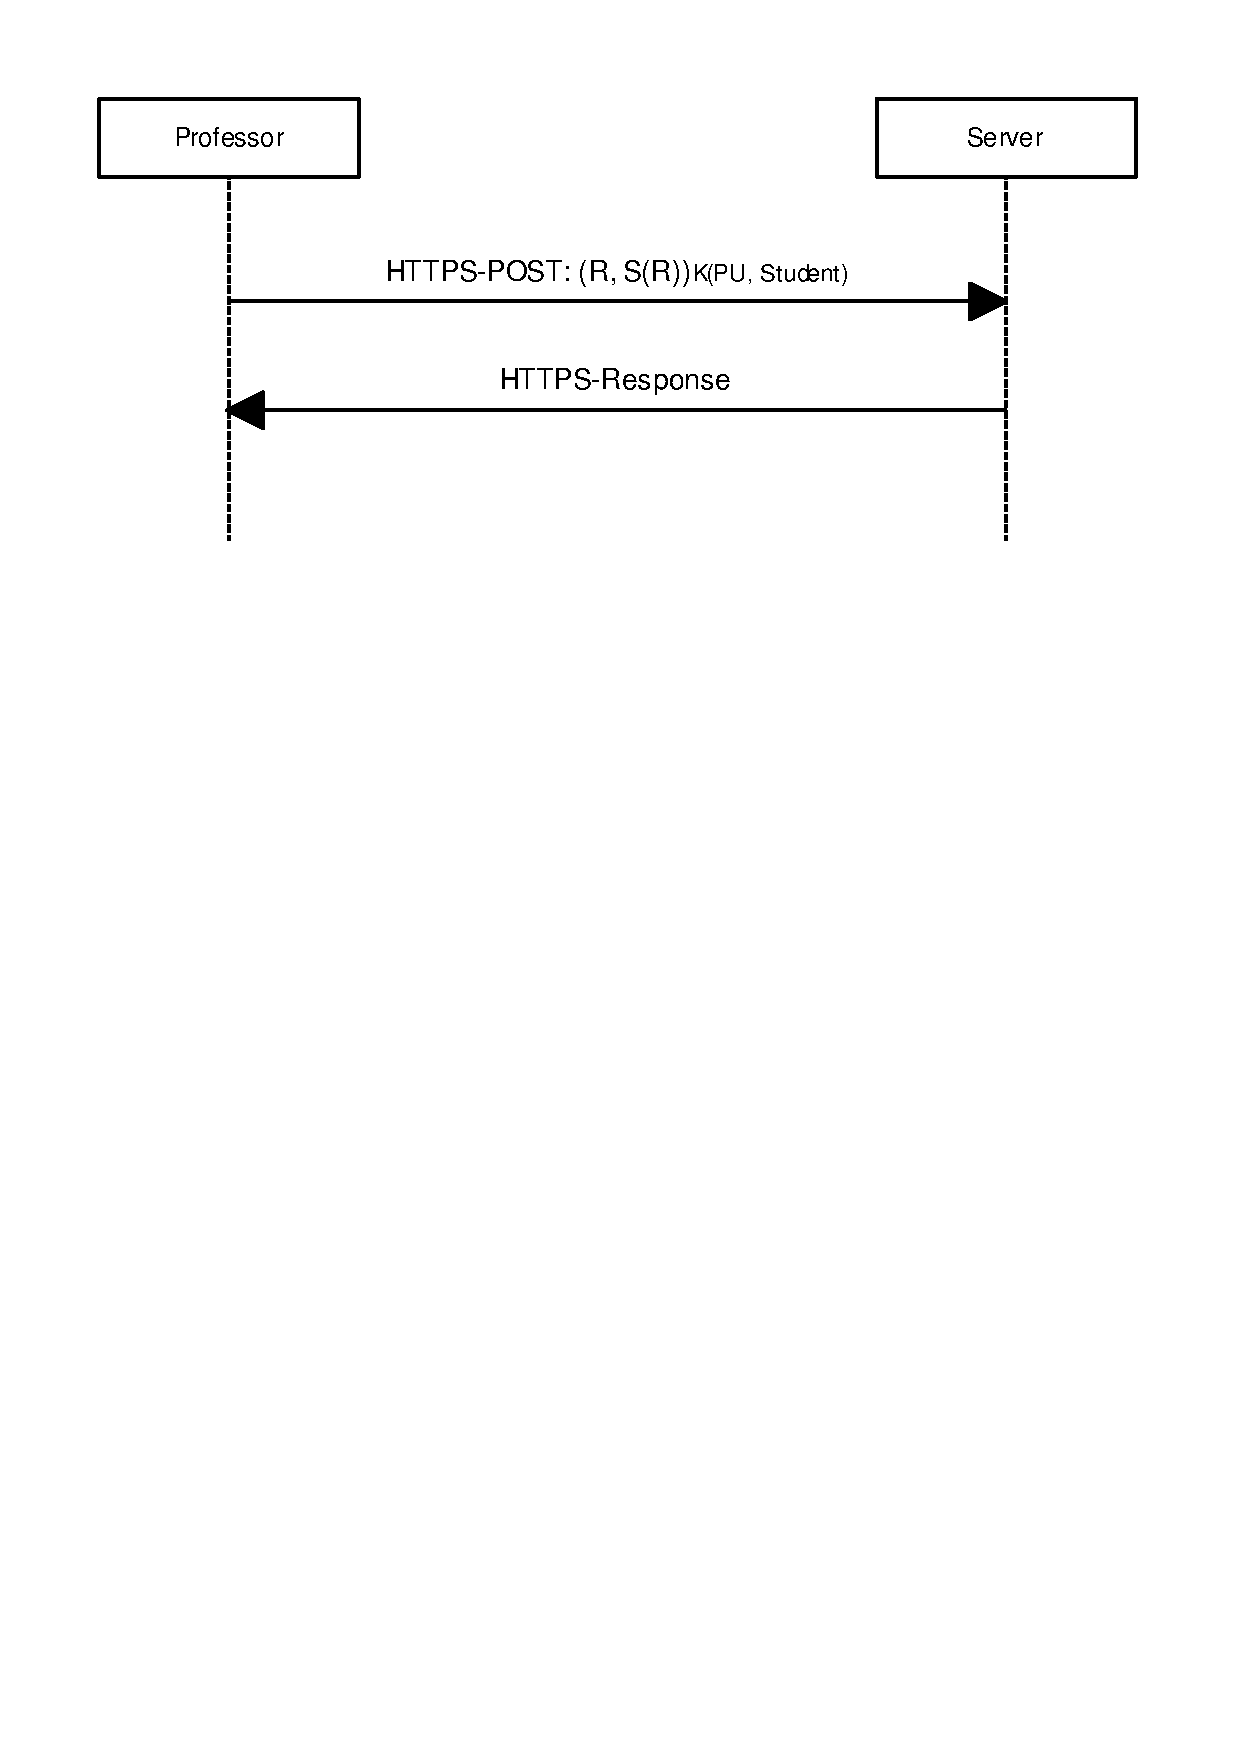
\includegraphics[width=\textwidth]{images/upload_scores.pdf}
\caption{Messages exchanged when uploading scores}
\label{fig:log-in}
\end{center}
\end{figure}

\begin{figure}
\begin{center}
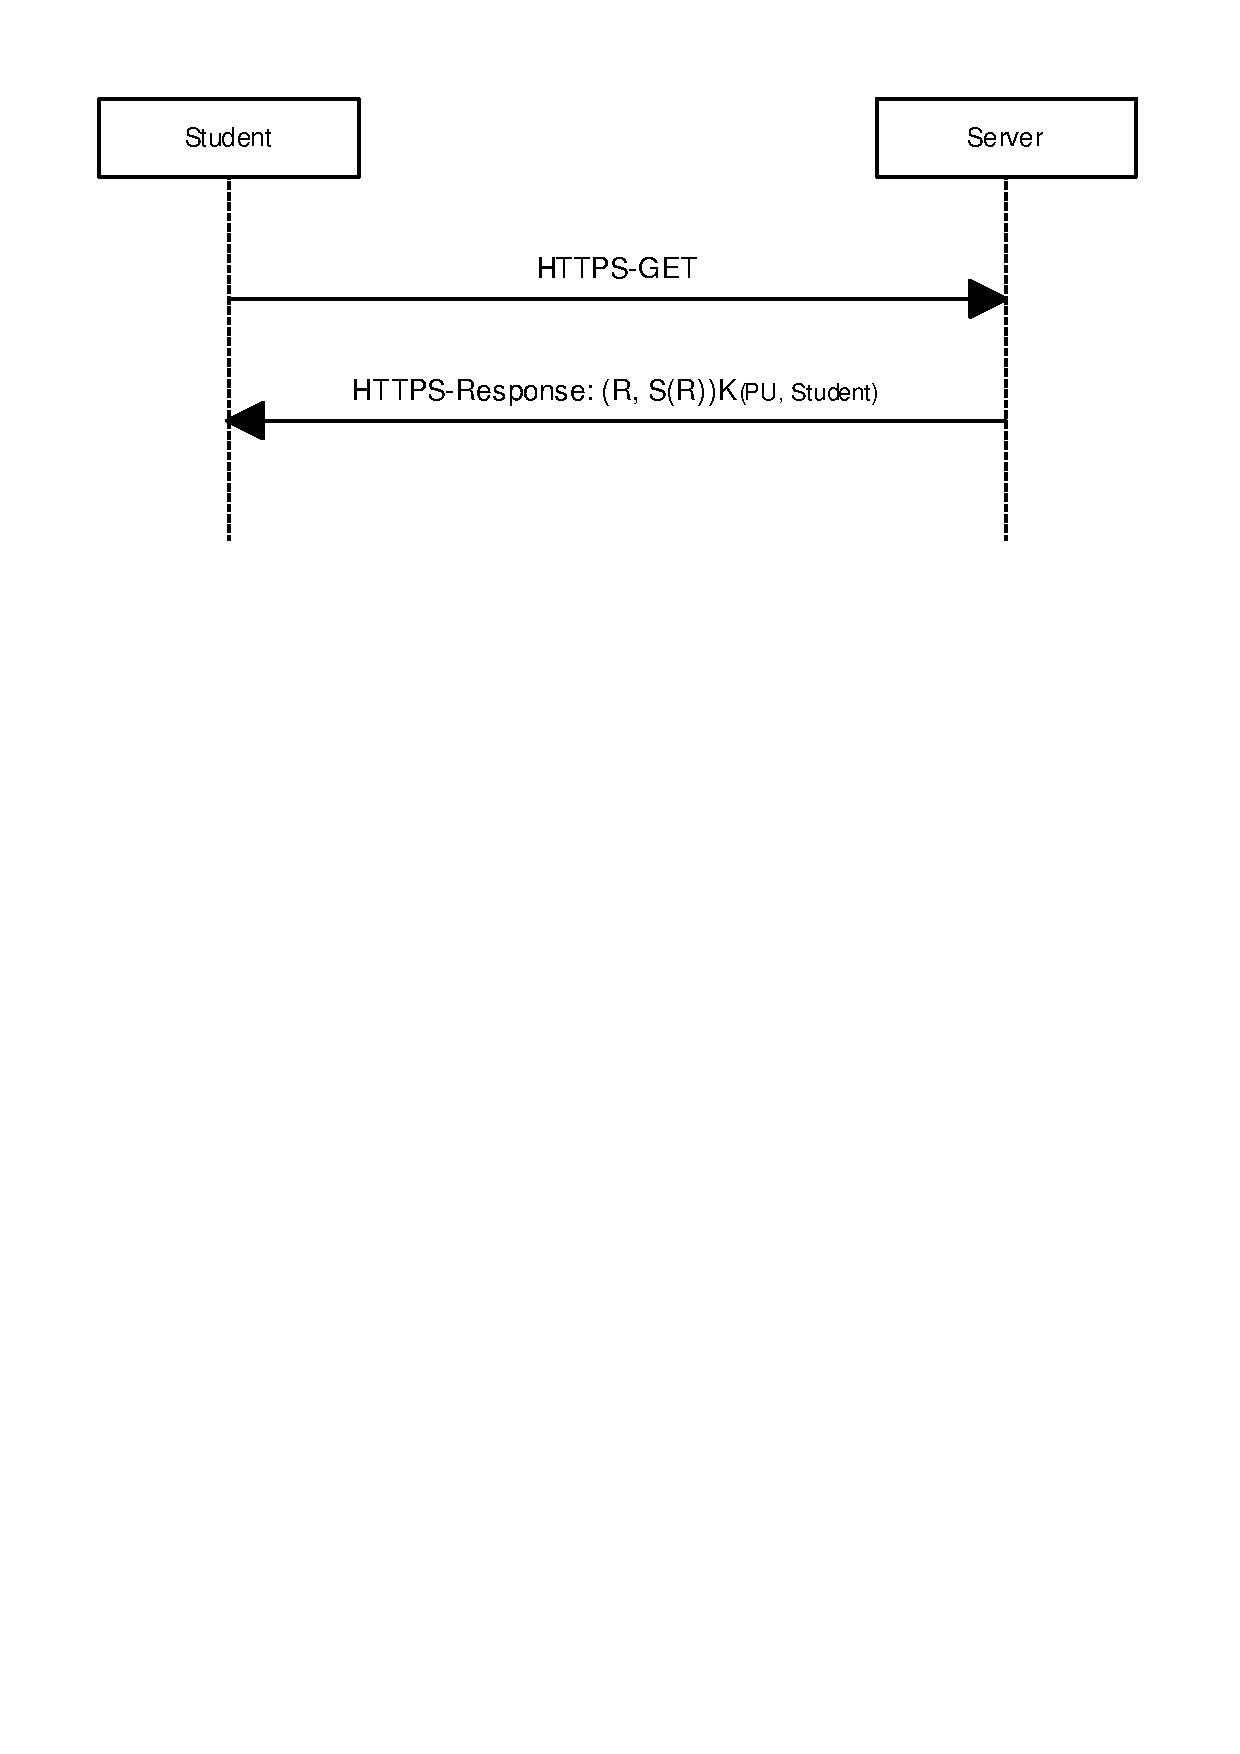
\includegraphics[width=\textwidth]{images/download_scores.pdf}
\caption{Messages exchanged when downloading scores}
\label{fig:log-in}
\end{center}
\end{figure}

+8000 words.

\end{document}
